206. \begin{figure}[ht!]
\center{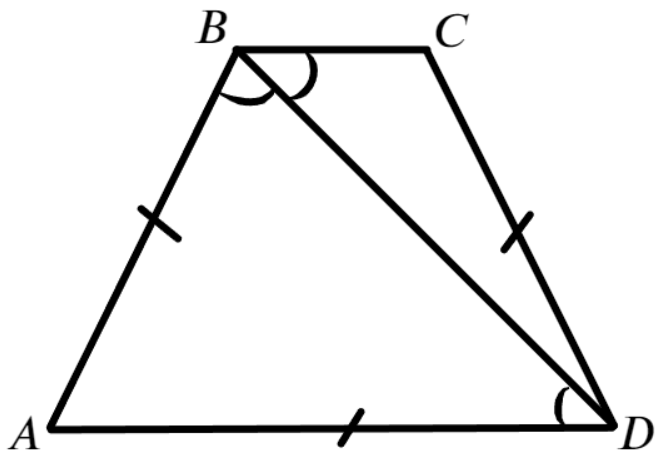
\includegraphics[scale=0.35]{g8-205.png}}
\end{figure}\\
Углы $DBC$ и $ADB$ равны как накрест лежащие при параллельных прямых $BC$ и $AD,$ поэтому $\angle ABD=\angle DBC=\angle ADB,$ треугольник $ABD$ является равнобедренным и $AD=AB=CD$ (так как трапеция равнобедренная). Пусть $AD=x,\ BC=y,$ тогда имеем систему\\ $\begin{cases} x+31=3x+y,\\ \cfrac{x+y}{2}=10. \end{cases}
\Leftrightarrow  \begin{cases} 2x+y=31,\\ x+y=20. \end{cases} \Rightarrow x=11$см.\\
